\chapter{Il criptosistema Merkle-Hellman} \label{ch:capitolo14}
\section{Il problema dello zaino (KNAPSACK}
\textbf{Input:} Gli interi positivi $v_1,v_2,...v_n$\\
\textbf{Output:} SI/NO secondo che esista una sequenza $e1,e_2....,e_n$ di bit 0,1
per cui:
\begin{figure}[htp]
    \centering
    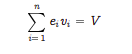
\includegraphics[scale=0.9]{tesi_stile/img/foto1cap14.png}
\end{figure}
\\\\\textbf{Teorema}\\
l problema KNAPSACK è NP-completo\\\\
\textbf{Dimostrazione}\\
\begin{itemize}
    \item KNAPSACK $\in$ NP. Invero
    
    \begin{figure}[htp]
        \centering
        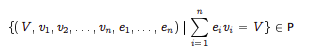
\includegraphics[scale=0.9]{tesi_stile/img/foto2cap14.png}
    \end{figure}
    
    \item Per provare KNAPSACK è NP-arduo, basta mostrare che 3SAT $<=_p$ KNAPSACK.
    
    \item Dobbiamo associare a ogni sistema di 3-clausole un’istanza di KNAPSACK, calcolabile in tempo polinomiale, in modo che sistemi soddisfacibili siano associati a elementi di KNAPSACK, e sistemi insoddisfacibili a elementi del suo complemento.
\end{itemize}
\textbf{Esempio}
 \begin{figure}[htp]
    \centering
    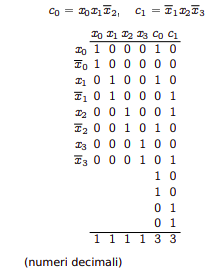
\includegraphics[scale=0.9]{tesi_stile/img/foto3cap14.png}
\end{figure}
\\Selezioniamo le righe corrispondenti ai letterali di una valutazione che soddisfa il sistema:\\
Ci sarà esattamente un 1 in ogni colonna $x_i$ e da uno a tre 1 nelle colonne $c_j$.
Aggiungendo qualcuna delle righe rimanenti otteniamo la soluzione di KNAPSACK
Viceversa, una soluzione di KNAPSACK seleziona le righe corrispondenti ai letterali di una
valutazione che soddisfa il sistema, più qualcuna delle righe ulteriori
\begin{center}
    \textbf{E' una riduzione polinomiale}
\end{center}
\newpage
\subsection{Crittografia}
\textbf{Due processi}
\begin{enumerate}
    \item Il mittente cifra il suo messaggio \textbf{(codifica)}
    
    \item Il destinatario decifra il testo originale \textbf{(decodifica)}
\end{enumerate}
\textbf{Esempio}\\
Codice cesareo
\begin{itemize}
    \item \textbf{Codifica:} $A \mapsto D, B \mapsto E, C \mapsto F, D \mapsto G, ...$
    
    \item \textbf{Decofica:} $A \mapsto U, B \mapsto V, C \mapsto Z, D \mapsto A, ...$
    
Lo scambio di chiavi è un aspetto critico
\end{itemize}
\textbf{Crittografia chiave pubblica}
\begin{itemize}
    \item Ogni utente dispone di due chiavi
    
        \begin{itemize}
            \item Una pubblica, con cui gli interlocutori cifrano i messaggi a lui destinati
            
            \item Una privata (segreta e personale) che serve per decifrarli
        \end{itemize}
    
    \item Chiunque può codificare, ma uno solo può decodificare
    
    \item Dalla funzione di codifica f non è facile calcolare la funzione di decodifica $f^{-1}$
\end{itemize}
\newpage
\subsection{Successioni supercrescenti}
\textbf{Definizione}\\
Una sequenza di interi $v_1, v_2, ... , v_n$ si dice supercrescente se
\begin{figure}[htp]
    \centering
    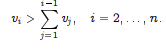
\includegraphics[scale=0.9]{tesi_stile/img/foto4cap14.png}
\end{figure}
Nel caso di sequenze supercrescenti, la soluzione di KNAPSACK è facile:
\begin{figure}[htp]
    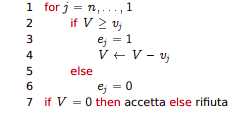
\includegraphics[scale=0.9]{tesi_stile/img/foto5cap14.png}
\end{figure}
\newpage
\textbf{Esempio}
\\La successione 2, 3, 7, 15, 31, 62 è supercrescente. 
\\Vediamo se $(24, 2, 3, 7, 15, 31, 62) \in$ KNAPSACK Poichè $24 < 62 e 24 < 31$, scartiamo 62 e 31.
\\Poi si ha 24 $>=$15 e 24 $-$ 15 $=$ 9.
\\Proseguendo, $9 >= 7$ e $9 - 7 = 2$ Ancora $2 < 3$, poi $2 >= 2$ e $2 - 2 = 0$.\\
In conclusione, $60 = 15 + 7 + 2$
\subsection{Creazione delle chavi}
\begin{itemize}
    \item Parto da una sequenza supercrescente $v_1, v_2, ... ,v_n$ , m e un intero a tale che gcd(m, a) = 1.
    
        \begin{center}
            $(w_1,w_2,...,w_n)$
        
        con $w_i = av_i$ mod m, i = 1,..., n
        \end{center}
        
    \item La chiave privata è 
        \begin{center}
            $(a', v_1, v_2,..., v_n )$
        \end{center}
    con a' inverso di a modulo m.
    
    \item Il messaggio è una sequenza di n bit $e_1,...,e_n$ che si codificherà con
    \begin{figure}[htp]
        \centering
        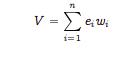
\includegraphics[scale=0.9]{tesi_stile/img/foto6cap14.png}
    \end{figure}
\end{itemize}
\textbf{Esempio}\\
Se la sequenza supercrescente è 2, 3, 7, 15, 31, 62 e a = 9 allora m = 62, a' = 7 e la chiave pubblica sarà
\begin{center}
    18, 27, 1, 11, 31
\end{center}
Il messaggio 10011 sarà codificato con
\begin{center}
    18 + 11 + 31 = 60
\end{center}
\newpage
\subsection{Decodifica}
\begin{itemize}
    \item Ricordiamo che
    
    \begin{figure}[htp]
        \centering
        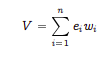
\includegraphics[scale=0.9]{tesi_stile/img/foto7cap14.png}
    \end{figure}
    
    \item Pertanto 
    
    \begin{figure}[htp]
        \centering
        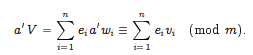
\includegraphics[scale=0.9]{tesi_stile/img/foto10cap14.png}
    \end{figure}

Tenendo conto del fatto che:
\begin{figure}[htp]
    \centering
    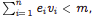
\includegraphics[scale=0.9]{tesi_stile/img/foto11cap14.png}
\end{figure}
    \item Conoscendo a' e V posso calcolare \textbf{la sommatoria precedente}

    \item Infine, per la supercrescenza delle $v_i$, posso ottenere rapidamente $e_1,...,e_n$\\\\
\end{itemize}
\textbf{Esempio}\\
Con la sequenza supercrescente è 2, 3, 7, 15, 31, a = 9, m = 62, a' = 7 riceviamo il messaggio V = 60.
\\Per prima cosa calcoliamo a'V mod m = 7 · 60 mod 62 = 48.
\\Con l’algoritmo per le successioni supercrescenti otteniamo
\begin{center}
    48 = 31 + 15 + 2
\end{center}
e quindi $e_1,e_2,e_3,e_4,e_5 = 10011$.
\newpage
\subsection{La classe UP}
\textbf{Definizione}\\
Una macchina di Turing non deterministica si dice non ambigua se ogni input al più una computazione convergente.
\\La classe dei problemi accettati da macchine di Turing non ambigue con
complessità temporale polinomiale si denota UP.
\\Il problema KNAPSACK appartiene alla classe UP
\begin{itemize}
    \item Non è noto se P = UP, né se NP = UP.
\end{itemize}